
\section{Load/Save data}

\begin{frame}[fragile]{File operations: Reading}

  Opening an existing file 

  \begin{minted}{python}
    >>> f = open("test.txt","rb")
    >>> print f
    <open file 'test.txt', mode 'rb' at 0x...>
  \end{minted}
  \bigskip
  \pause
  Reading it:
  \begin{minted}{python}
    >>> f.read()
    'hello world'
  \end{minted}
  \pause
  \bigskip
  Closing it:
  \begin{minted}{python}
    >>> f.close()
    >>> print f
    <closed file 'test.txt', mode 'rb' at 0x...>
  \end{minted}

\end{frame}


\begin{frame}[fragile]{File operations: Writing}

  Opening a (new) file 

  \begin{minted}{python}
    >>> f = open("new_test.txt","wb")
    >>> print f
    <open file 'test.txt', mode 'wb' at 0x...>
  \end{minted}
  \bigskip
  \pause
  Writing to it:
  \begin{minted}{python}
    >>> f.write("hello world, again")
    >>> f.write("... and again")
    >>> f.close()
  \end{minted}
  \pause
  \vspace{0.65cm}

  \begin{arrowlist}
  \item Only after calling close() the changes appear in the file for
    editing elsewhere!
  \end{arrowlist}

\end{frame}

\begin{frame}[fragile]{File operations: Appending}

  Opening an existing file 

  \begin{minted}{python}
    >>> f = open("test.txt","ab")
    >>> print f
    <open file 'test.txt', mode 'ab' at 0x...>
  \end{minted}
  \bigskip
  \pause  

  Appending to it:
  \begin{minted}{python}
    >>> f.write("hello world, again")
    >>> f.write("... and again")
    >>> f.close()
  \end{minted}
  \pause
  \vspace{0.8cm}

  \begin{arrowlist}
  \item In append mode the \textbf{file pointer} is set to the end of the opened file.
  \end{arrowlist}

\end{frame}


\begin{frame}[fragile]{File operations: More about file pointers}

  \begin{mlinepython}
    f = open("lines_test.txt", "wb")
    for i in range(10):
        f.write("this is line %d \n" %(i+1))
    f.close()
  \end{mlinepython}
  \pause
  \bigskip

  Reading from the file:
  \smallskip

  \begin{minted}{python}
    >>> f = open("lines_test.txt", "rb")
    >>> f.readline()
  \end{minted}
  \pause
  \vspace{-10pt}
  \begin{minted}{python}
    'this is line 1 \n'
  \end{minted}
  \pause
  \vspace{-10pt}
  \begin{minted}{python}
    >>> f.readline()
  \end{minted}
  \pause
  \vspace{-10pt}
  \begin{minted}{python}
    'this is line 2 \n'
  \end{minted}
  \pause
  \vspace{-10pt}
  \begin{minted}{python}
    >>> f.read(14)
  \end{minted}
  \pause
  \vspace{-10pt}
  \begin{minted}{python}
    'this is line 3'
  \end{minted}
  \pause
  \vspace{-10pt}
  \begin{minted}{python}
    >>> f.read(2)
  \end{minted}
  \pause
  \vspace{-10pt}
  \begin{minted}{python}
    ' \n'
  \end{minted}

\end{frame}


\begin{frame}[fragile]{File operations: More about file pointers}

  \begin{mydescription}{wbsssssssssssssssssssssssss}
    \itemsep4pt
    \item<1->[\texttt{f.tell()}] gives current position within file~\textbf{\texttt{f}}
    \item<2->[\texttt{f.seek(x[, from])}] change file pointer
      position within file~\textbf{\texttt{f}}, where 
      \hspace{0.2cm}\begin{mydescription}{wbssssssss}
        \itemsep0pt
        \item[\normalfont{from = 0}] from beginning of file
        \item[\normalfont{from = 1}] from current position
        \item[\normalfont{from = 2}] from end of file
      \end{mydescription}
  \end{mydescription}

  \bigskip
  \medskip
  \onslide<3->

  \begin{mlinepython}
    >>> f = open("lines_test.txt", "rb")
    >>> f.tell()
    0
    >>> f.read(10)
    'this is li'
    >>> f.tell()
    10
  \end{mlinepython}

\end{frame}


\begin{frame}[fragile]{File operations: More about file pointers}
  \begin{mlinepython}
    >>> f.seek(5)
    >>> f.tell()
    5
    >>> f.seek(10,1)
    >>> f.tell()
    15
    >>> f.seek(-10,2)
    >>> f.tell()
    151
    >>> f.read()
    ' line 10 \n'
  \end{mlinepython}
\end{frame}

%

\begin{frame}[fragile]{File operations: Other Modes}
  %\stretchy

  \begin{mydescription}{wbssssssss}
    \itemsep22pt
    \item<1->[rb+] Opens the file for reading and writing. File
      pointer will be at the beginning of the file.
    \item<2->[wb+] Opens for reading and writing. Overwrites the
      existing file if the file exists, otherwise a new file is created.
    \item<3->[ab+] Opens the file for appending and reading. The file
      pointer is at the end of the file if the file exists, otherwise
      a new file is created for reading and writing.
  \end{mydescription}

\end{frame}


\begin{frame}[fragile]{Saving Data: Python Pickle}

  \onslide<1->
  Use pickle to save and retrieve more complex data types - lists,
  dictionaries and even class objects:

  \bigskip\pause

  \onslide<2|handout:0>
  \begin{figure}
    \centering
    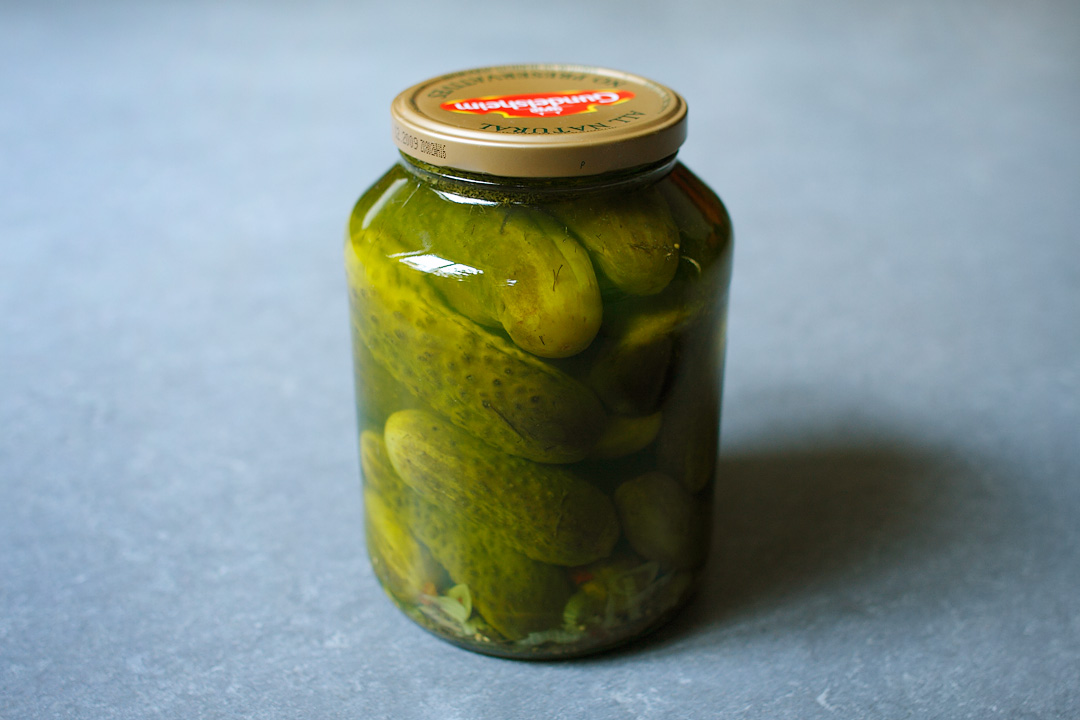
\includegraphics[width=6cm]{pickle.jpg}
    \caption*{\scriptsize  \textcopyright Dom Dada \href{http://creativecommons.org/licenses/by-nc-nd/2.0/}{CC BY-NC-ND 2.0}}
  \end{figure}
  
  \vspace{-5.6cm}
  \onslide<3->
  \begin{mlinepython}
    >>> import pickle 
    >>> f = open('save_file.p', 'wb')
    >>> ex_dict = {'hello': 'world'}
    >>> pickle.dump(ex_dict, f)
    >>> f.close()
  \end{mlinepython}

  \bigskip\onslide<4->

  \begin{mlinepython}
    >>> import pickle 
    >>> f = open('save_file.p', 'rb')
    >>> loadobj = pickle.load(f)
    >>> print loadobj['hello']
    world
  \end{mlinepython}

\end{frame}


\begin{frame}[fragile]{Best practice: With Statement}


  \begin{mlinepython}
    import pickle 

    ex_dict = {'hello': 'world'}

    with open('save_file.p', 'wb') as f:
        pickle.dump(ex_dict, f)
  \end{mlinepython}

  \bigskip \pause
  \vspace{0.2cm}

  \begin{mlinepython}
    import pickle 

    with open('save_file.p', 'rb') as f:
        loadobj = pickle.load(f)

    print loadobj['hello']
  \end{mlinepython}
  \vspace{0.15cm}
  \begin{arrowlist}
  \item Use this!
  \end{arrowlist}

\end{frame}


%%% Local Variables: 
%%% mode: latex
%%% TeX-master: "data_processing"
%%% End: 
